\chapter{結果と評価}
\label{chap:results}
本章では,3章で紹介した手法によって自動生成した吹奏アニメーションについて記述する.
\secref{sec:system}ではシステムの仕様や使用したPCについて述べ,
\secref{sec:result}では自動生成した吹奏アニメーションのキャプチャリング画像を示す.
そして\secref{sec:review}では,自動生成結果を実際の演奏シーンや既存の吹奏アニメーションと比較することにより,提案手法を評価する.

\section{実行環境} \label{sec:system}
事前にUnreal Engineにて専用のプロジェクトを作成し,モーションのデータが記載されているUnreal Engine専用のファイルをインポートする.
そして,キャラクタと,それぞれが演奏する楽器を\figref{fig:ue4}のようにセッティングする.
なお,最初にインポートするUnreal Engine専用のファイルには,キャラクタの姿勢データも存在するため,
キャラクタの姿勢のセッティングは容易にできる.\\
\indent
実装環境は\tabref{tab:pc}の通りである.
\begin{figure}[h]
	\centering
	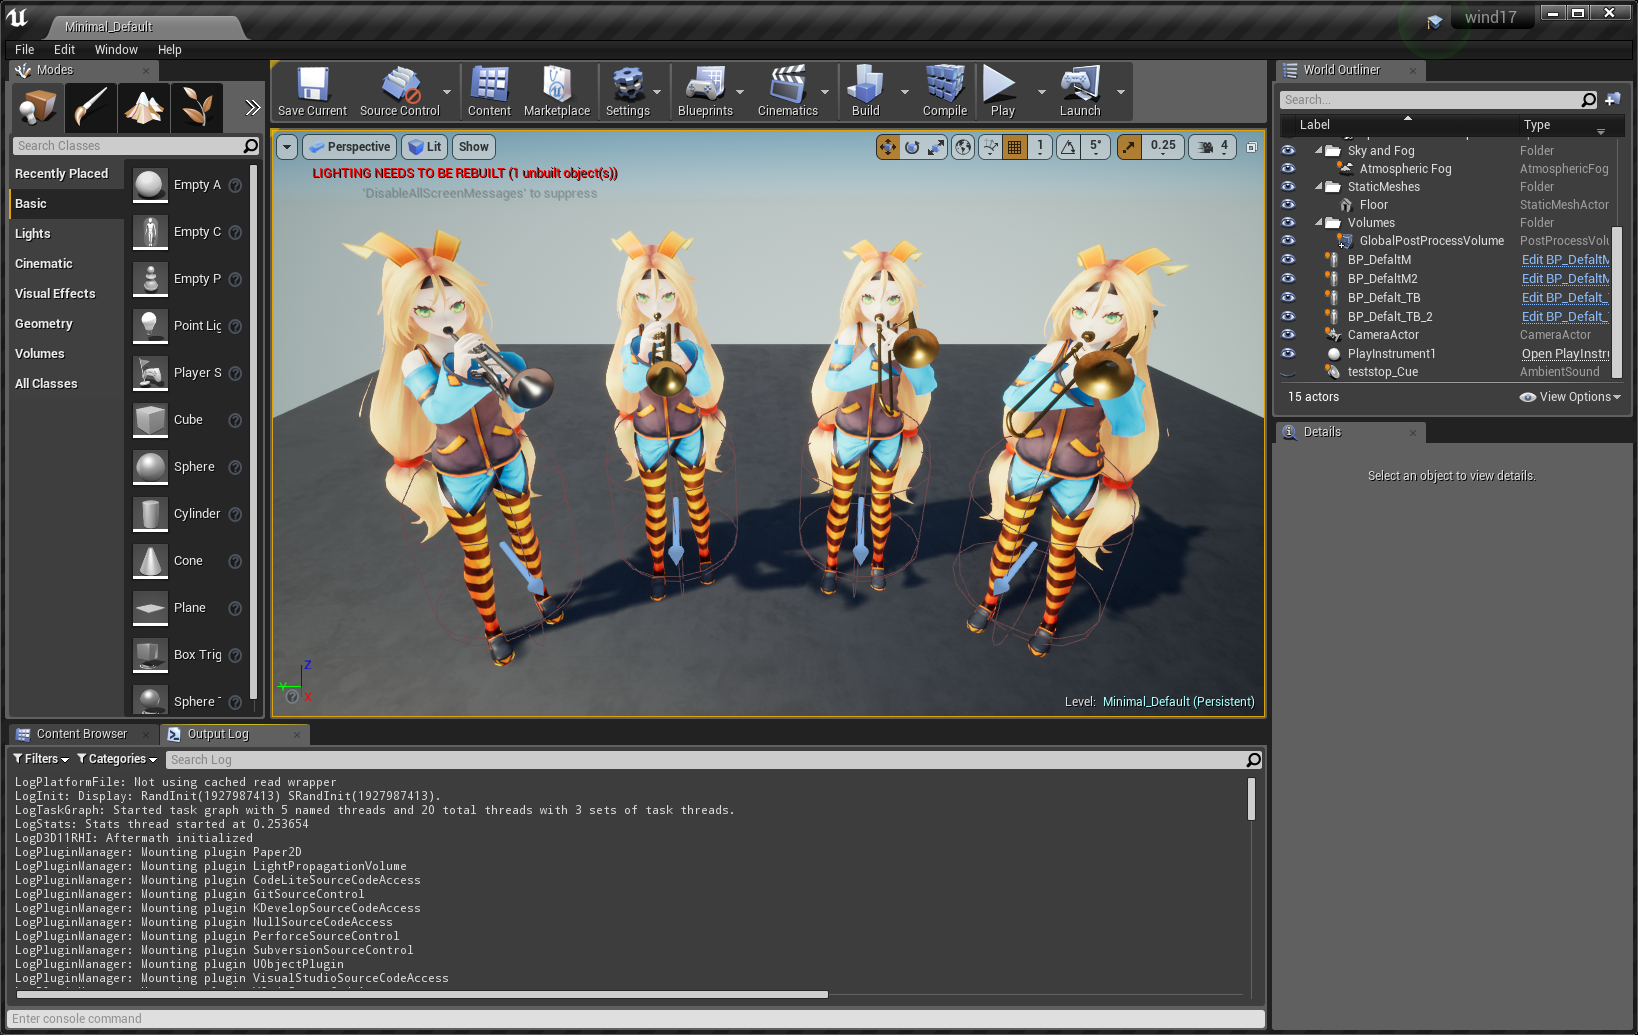
\includegraphics[width=14cm]{fig/chap4/ue4.eps}
	\caption{Unreal Engineの初期設定画面}
	\label{fig:ue4}
\end{figure}

\begin{table}[htbp] 
	\begin{center}
		\caption{実装環境}
		\label{tab:pc}
		\begin{tabular}{|l|c|}
			\hline
			OS & Windows10 64bit \\ \hline
			CPU & Intel\textregistered Core\textsuperscript{TM}i7-3930K \\ \hline
			RAM & 32.00GB\\ \hline
			言語 & c++\\ \hline
		\end{tabular}
	\end{center}
\end{table}

\section{アニメーション自動生成結果} \label{sec:result}
本節では,自動生成したトランペット奏者2名で演奏するアンサンブルアニメーションと,トランペット奏者2名,トロンボーン奏者2名の計4名で演奏するアンサンブルアニメーションのキャプチャリング画像を示し,自動生成結果について述べる.
以下,2つのアニメーションそれぞれについて,制御している口元やボーンを示すが,
前者のアニメーションでは,トランペット奏者の口元や指元がズームインされているため,主に口元や指元のボーンの制御に,
後者のアニメーションでは,全体を俯瞰しているシーンであるため,前者のアニメーションにて触れなかったボーンの制御に触れる.\\
\indent
まず,トランペット奏者2名でのアンサンブルアニメーションの自動生成結果について述べる.
\figref{fig:anim1}は,基本姿勢である.
\begin{figure}[!h]
	\centering
	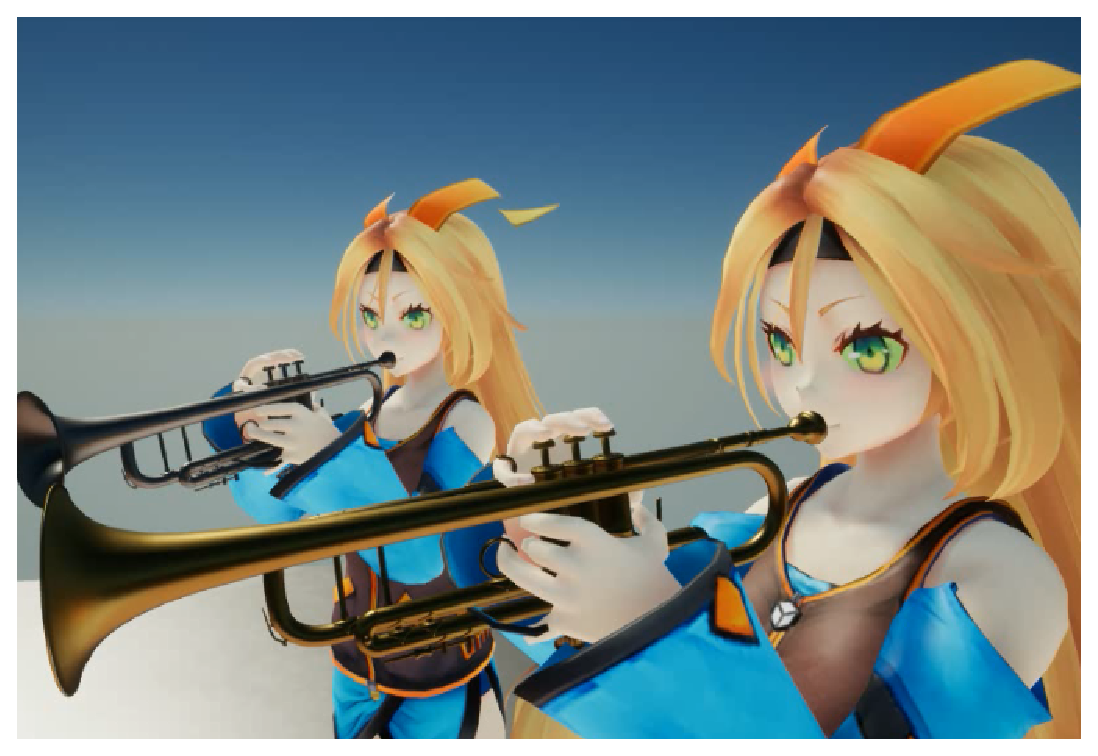
\includegraphics[width=10cm]{fig/chap4/anim1.eps}
	\caption{トランペット奏者2名の基本姿勢}
	\label{fig:anim1}
\end{figure}
\\
トランペットを演奏する際は,\figref{fig:anim1_finger}のように指でピストンを操作する.
\begin{figure}[!h]
	\centering
	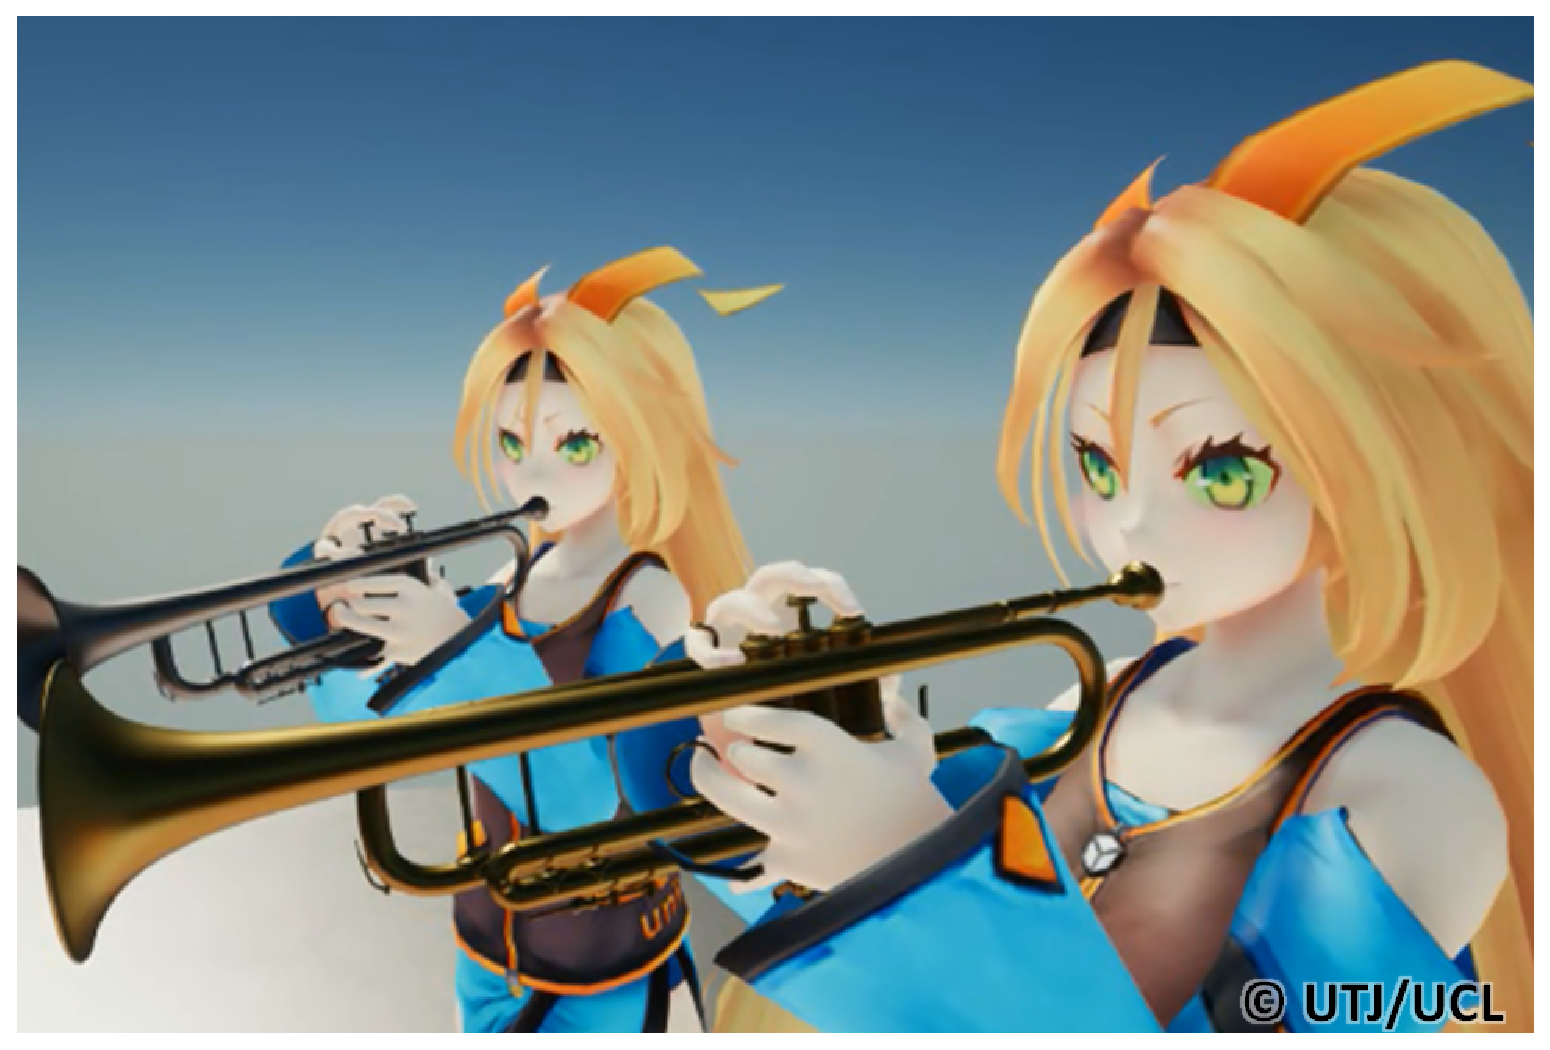
\includegraphics[width=10cm]{fig/chap4/anim1_finger.eps}
	\caption{トランペット奏者がピストンを押す様子}
	\label{fig:anim1_finger}
\end{figure}
\\
%\newpage
息継ぎをするタイミングでは,演奏者は\subfigref{fig:zoom}{fig:zoom_breath}のように口を開ける.
また,高音を演奏するタイミングでは,\subfigref{fig:zoom}{fig:zoom_high}のように口元が緊張する.
\vspace{-2mm}
\begin{figure}[h]
	\centering
	\subcaptionbox{\textgt{息継ぎをしている様子}
		\label{fig:zoom_breath}}[0.45\linewidth]{
		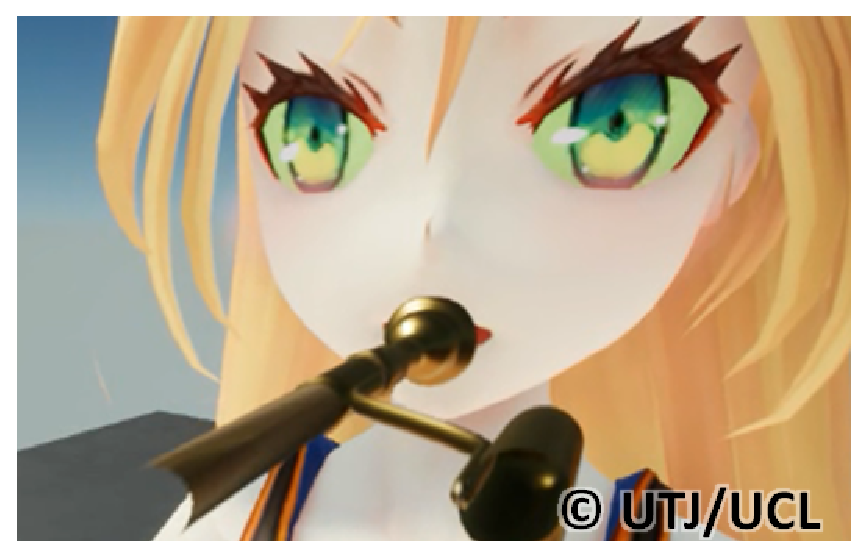
\includegraphics[width=5.5cm]{fig/chap4/anim1_zoom_breath.eps}}
	\subcaptionbox{\textgt{高い音を演奏し口元が緊張している様子}
		\label{fig:zoom_high}}[0.45\linewidth]{
		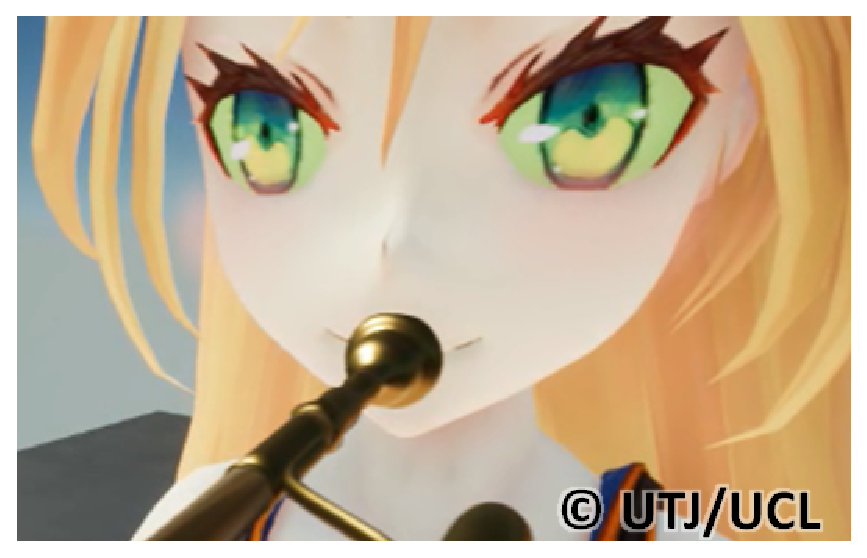
\includegraphics[width=5.5cm]{fig/chap4/anim1_zoom_high.eps}}
	\subcaptionbox{\textgt{通常の口元の様子}
		\label{fig:zoom_default}}[0.45\linewidth]{
		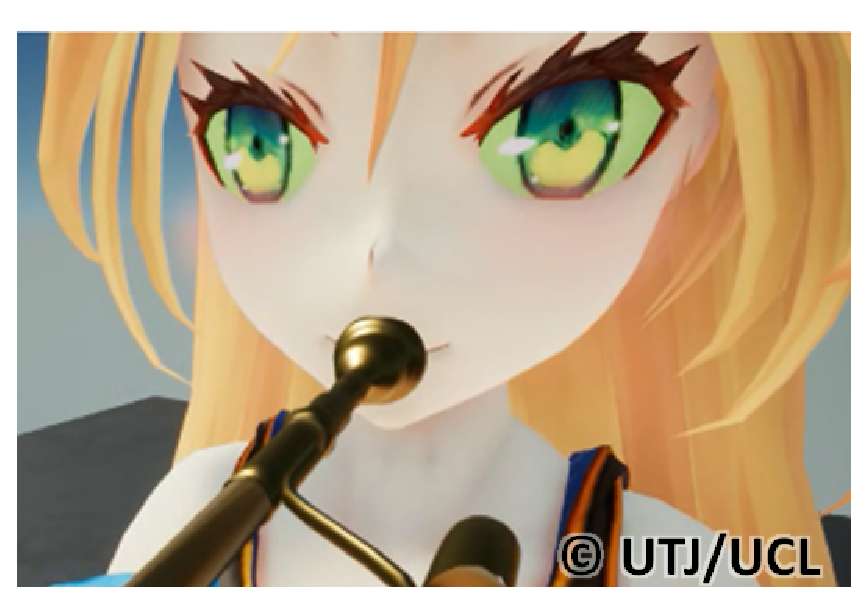
\includegraphics[width=5.5cm]{fig/chap4/anim1_zoom.eps}}
	\caption{演奏者の口元の様子}
	\label{fig:zoom}
\end{figure}
\\
\indent
次に,トランペット奏者2名,トロンボーン奏者2名でのアンサンブルアニメーションの自動生成結果について述べる.
\figref{fig:anim2}は,基本姿勢である.
\begin{figure}[h]
	\centering
	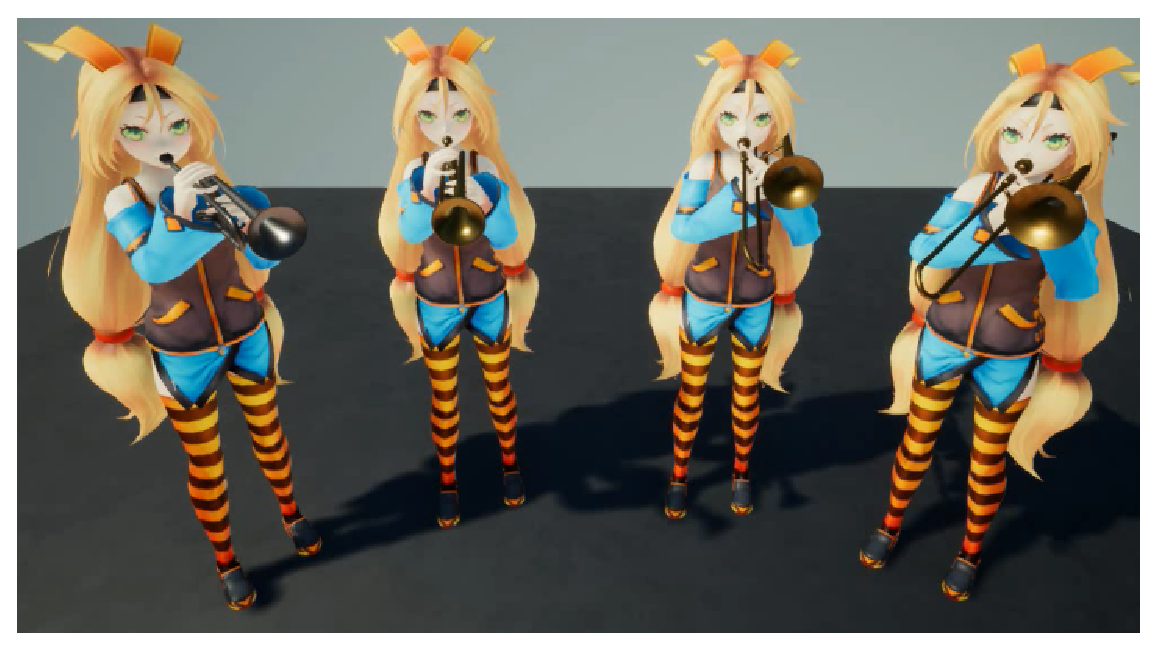
\includegraphics[width=13cm]{fig/chap4/anim2.eps}
	\caption{トランペット奏者2名とトロンボーン奏者2名の基本姿勢}
	\label{fig:anim2}
\end{figure}
\newpage
トロンボーンを演奏する際は,\figref{fig:anim2_slide}のように右手でスライドを操作する.
\begin{figure}[h]
	\centering
	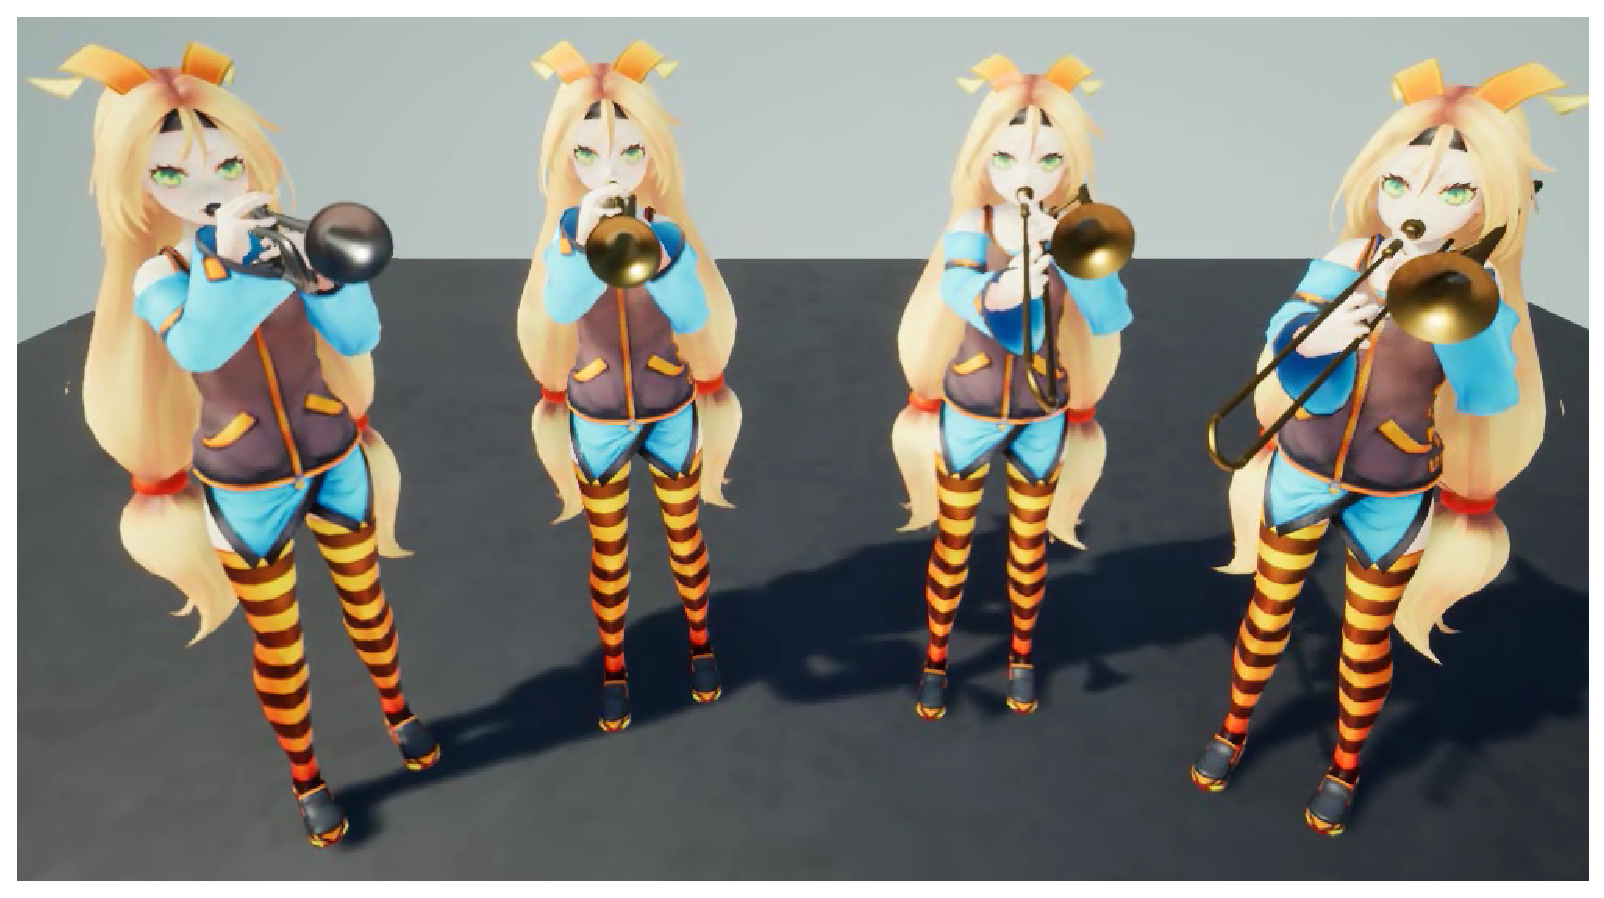
\includegraphics[width=13cm]{fig/chap4/anim2_slide.eps}
	\caption{トロンボーン奏者がスライドを動かす様子}
	\label{fig:anim2_slide}
\end{figure}
\\
曲の入りでは,タイミングを合わせるために,膝を使って楽器を縦に振る.
\figref{fig:anim2_down}は,膝を曲げ,楽器を下に向けた瞬間の様子である.
\begin{figure}[h]
	\centering
	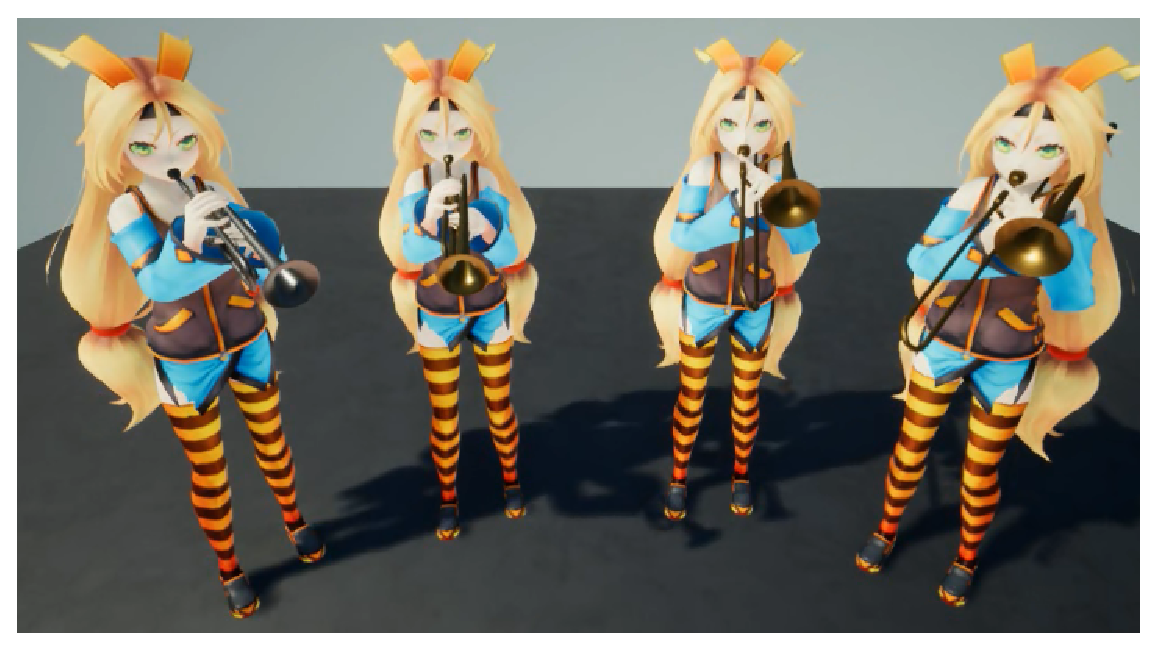
\includegraphics[width=13cm]{fig/chap4/anim2_down.eps}
	\caption{曲の入りを合わせるために膝を使い楽器を下に向けた瞬間の様子}
	\label{fig:anim2_down}
\end{figure}
\\
息継ぎをするタイミングでは,演奏者は身体を反らす.
\figref{fig:anim2_breath}は,トランペット奏者2名が息継ぎをしている瞬間の様子である.
\begin{figure}[h]
	\centering
	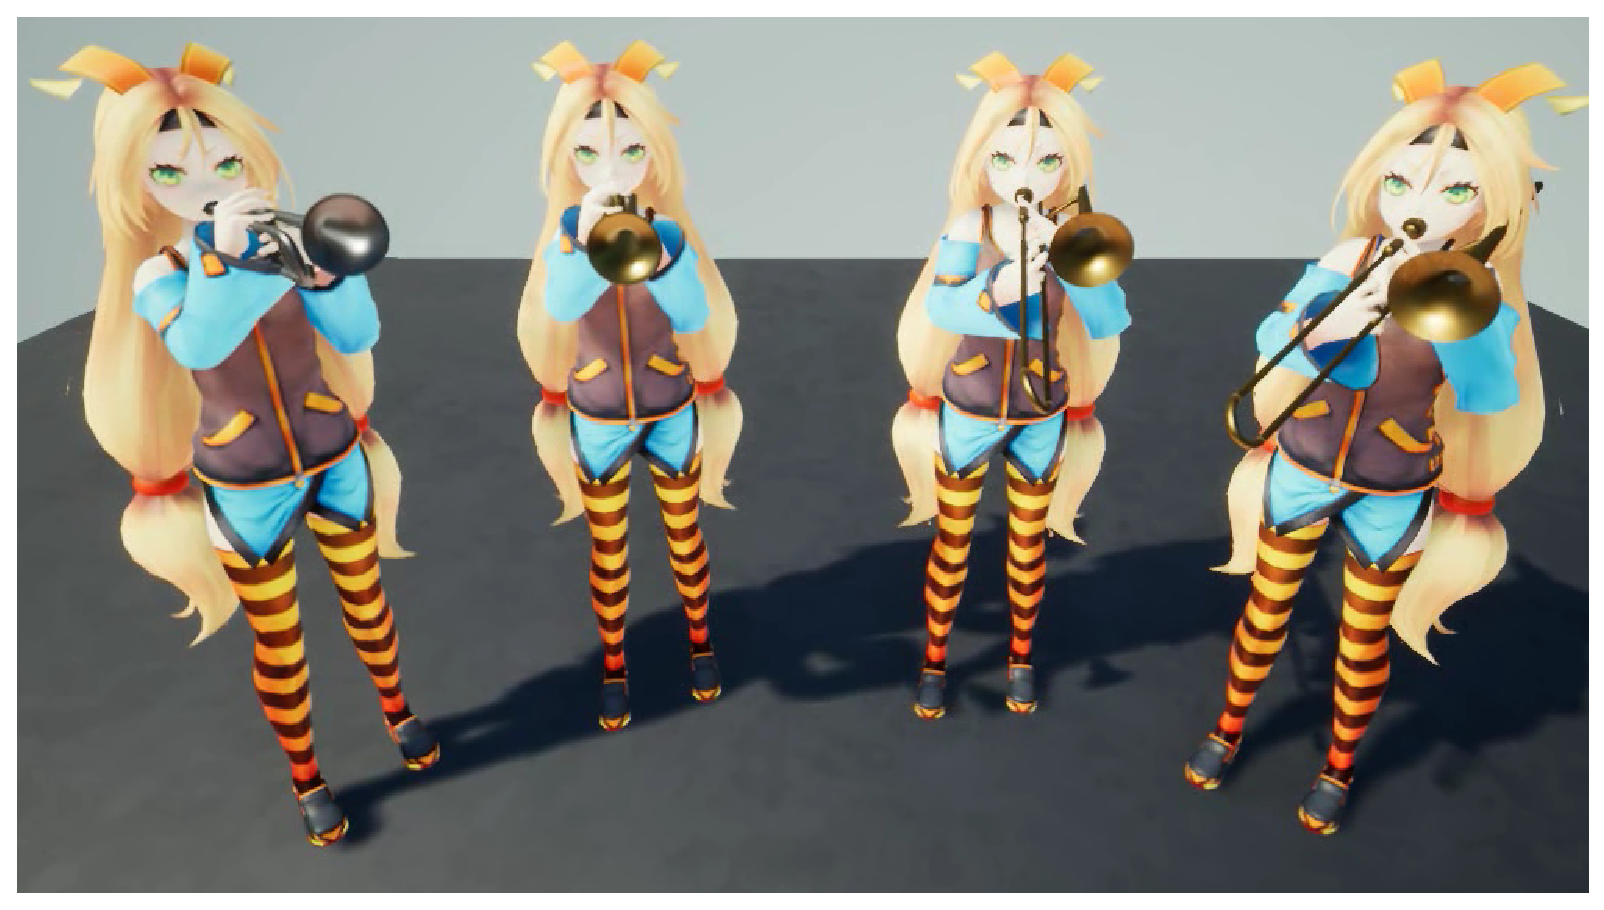
\includegraphics[width=13cm]{fig/chap4/anim2_breath.eps}
	\caption{息継ぎ時に身体を反らしている様子}
	\label{fig:anim2_breath}
\end{figure}
\newpage
\section{評価} \label{sec:review}
自動生成した吹奏アニメーションに対して,以下の3つの評価を行った.
\begin{itemize}
	\item 実際の演奏シーンとの比較による評価
	\item 既存のアニメーションとの比較による評価
	\item アンサンブルアニメーションの評価
\end{itemize}
以下,評価結果を,(a)吹奏楽・オーケストラ団体への所属経験者または金管楽器(主にトランペット,トロンボーン,ホルン,ユーフォニアム,チューバ)経験者10名の回答,(b)(a)にはあてはまらない楽器経験者13名の回答,(c)楽器未経験者9名の回答に分けて示す.

\newpage
\subsection{実際の演奏シーンとの比較による評価}
トランペット奏者やトロンボーン奏者が実際に演奏しているシーンと,自動生成した吹奏アニメーションを比較することによる評価を,以下の4項目について行った.
\begin{itemize}
	\item トランペット奏者の指の動きは再現できているか
	\item トランペット奏者の身体の動きは自然か
	\item トロンボーン奏者の腕の動きは再現できているか
	\item トロンボーン奏者の身体の動きは自然か
\end{itemize}
\vspace{5mm}
\par
\figref{fig:Q1-1}は,トランペット奏者の指の動きが再現できているか否かを評価した結果である.
吹奏楽やオーケストラ団体への所属経験や楽器の経験に関わらず,提案手法に対して肯定的な回答をした者がほとんどであり,否定的な回答をした者はいなかった.
\begin{figure}[!h]
	\centering
	\subcaptionbox{\textgt{吹奏楽・オーケストラ団体への所属経験者または金管楽器経験者の回答}
		\label{fig:Q1-1-1}}{
		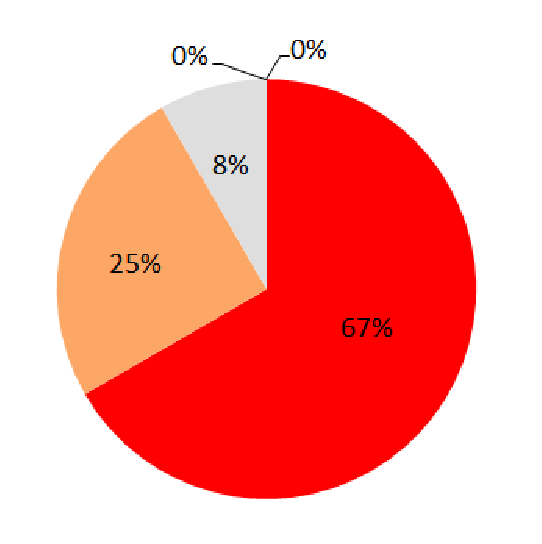
\includegraphics[width=4.8cm]{fig/chap4/Q1-1-1.eps}}
	\subcaptionbox{\textgt{(a)にはあてはまらない楽器経験者の回答}
		\label{fig:Q1-1-2}}{
		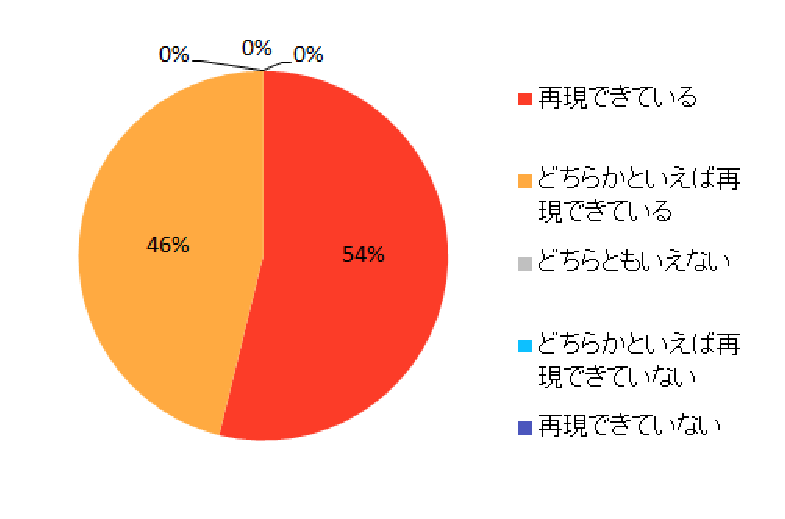
\includegraphics[width=4.8cm]{fig/chap4/Q1-1-2.eps}}
	\subcaptionbox{\textgt{楽器未経験者の回答}
		\label{fig:Q1-1-3}}{
		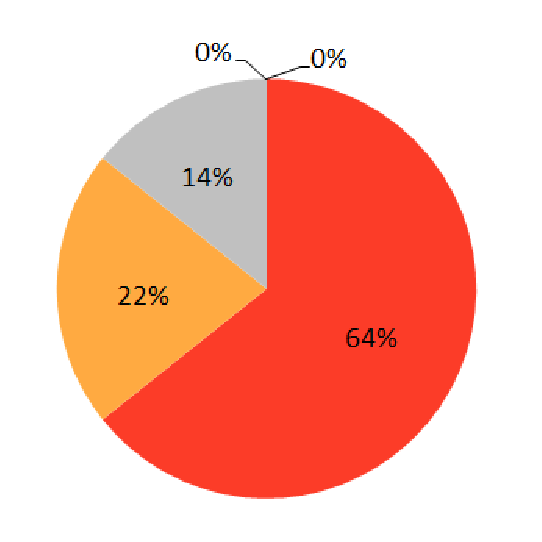
\includegraphics[width=4.8cm]{fig/chap4/Q1-1-3.eps}}
	\caption{トランペット奏者の指の動きは再現できているか}
	\label{fig:Q1-1}
\end{figure}
\vspace{5mm}
\par
\figref{fig:Q1-2}は,トランペット奏者の身体の動きが自然か否かを評価した結果である.
吹奏楽やオーケストラ団体への所属経験や楽器の経験に関わらず,提案手法に対して否定的な回答をした者の比率が高かった.
特に,楽器未経験者の比率が高かった.
\begin{figure}[!h]
	\centering
	\subcaptionbox{\textgt{吹奏楽・オーケストラ団体への所属経験者または金管楽器経験者の回答}
		\label{fig:Q1-2-1}}{
		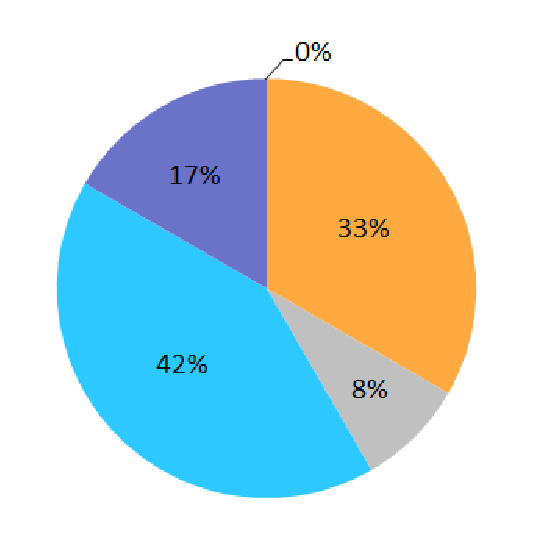
\includegraphics[width=4.8cm]{fig/chap4/Q1-2-1.eps}}
	\subcaptionbox{\textgt{(a)にはあてはまらない楽器経験者の回答}
		\label{fig:Q1-2-2}}{
		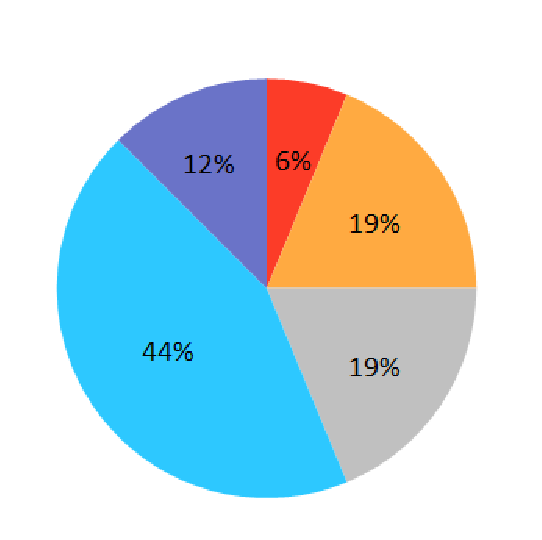
\includegraphics[width=4.8cm]{fig/chap4/Q1-2-2.eps}}
	\subcaptionbox{\textgt{楽器未経験者の回答}
		\label{fig:Q1-2-3}}{
		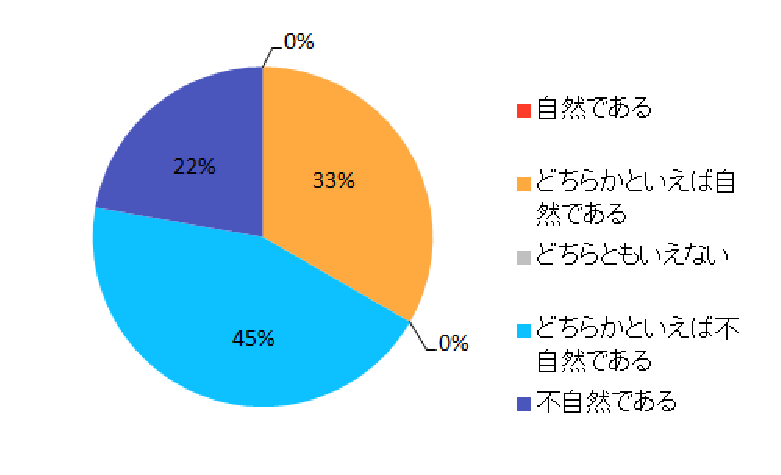
\includegraphics[width=4.8cm]{fig/chap4/Q1-2-3.eps}}
	\caption{トランペット奏者の身体の動きは自然か}
	\label{fig:Q1-2}
\end{figure}
\newpage
\par
\figref{fig:Q1-3}は,トロンボーン奏者の腕の動きが再現できているか否かを評価した結果である.
吹奏楽やオーケストラ団体への所属経験者や金管楽器奏者は,全員提案手法に対して肯定的な回答をした.
また,上記にあてはまらない者も,大半が肯定的な回答をした.
\begin{figure}[!h]
	\centering
	\subcaptionbox{\textgt{吹奏楽・オーケストラ団体への所属経験者または金管楽器経験者の回答}
		\label{fig:Q1-3-1}}{
		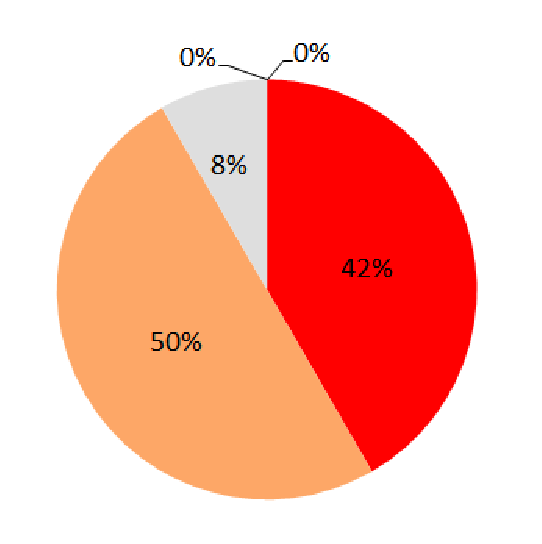
\includegraphics[width=4.8cm]{fig/chap4/Q1-3-1.eps}}
	\subcaptionbox{\textgt{(a)にはあてはまらない楽器経験者の回答}
		\label{fig:Q1-3-2}}{
		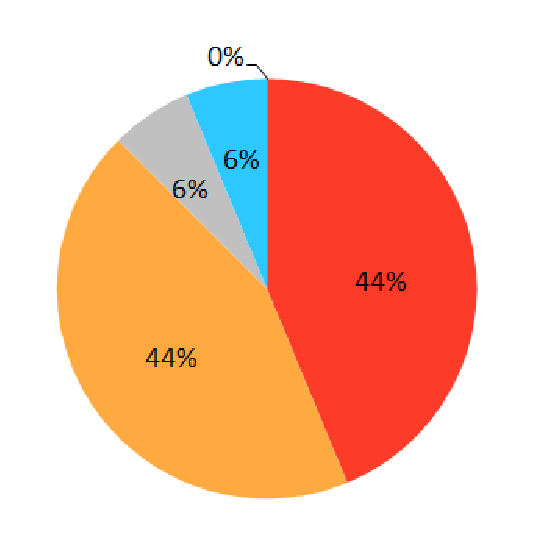
\includegraphics[width=4.8cm]{fig/chap4/Q1-3-2.eps}}
	\subcaptionbox{\textgt{楽器未経験者の回答}
		\label{fig:Q1-3-3}}{
		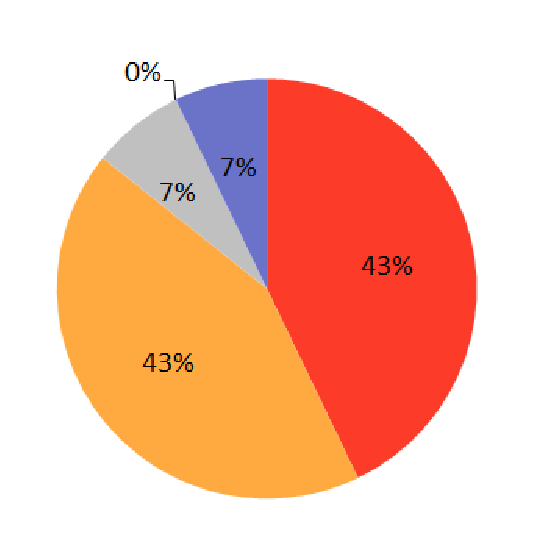
\includegraphics[width=4.8cm]{fig/chap4/Q1-3-3.eps}}
	\caption{トロンボーン奏者の腕の動きは再現できているか}
	\label{fig:Q1-3}
\end{figure}
\vspace{5mm}
\par
\figref{fig:Q1-4}は,トロンボーン奏者の身体の動きが自然か否かを評価した結果である.
提案手法に対して肯定的な回答をした者も否定的な回答をした者も,半数以下という結果になった.
また,楽器経験者より楽器未経験者の方が,肯定的な回答をした者の比率が高かった.
\begin{figure}[!h]
	\centering
	\subcaptionbox{\textgt{吹奏楽・オーケストラ団体への所属経験者または金管楽器経験者の回答}
		\label{fig:Q1-4-1}}{
		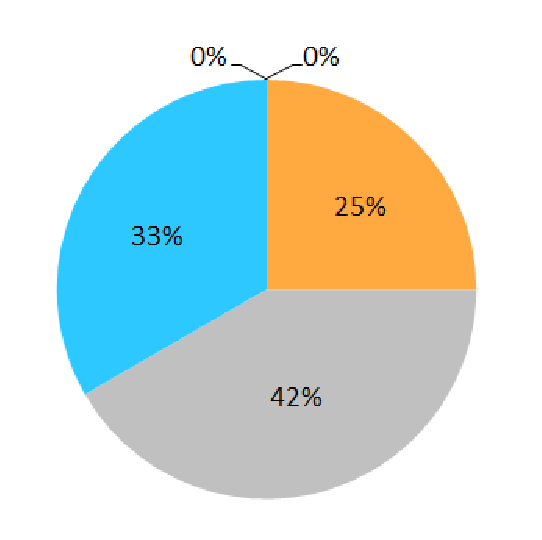
\includegraphics[width=4.8cm]{fig/chap4/Q1-4-1.eps}}
	\subcaptionbox{\textgt{(a)にはあてはまらない楽器経験者の回答}
		\label{fig:Q1-4-2}}{
		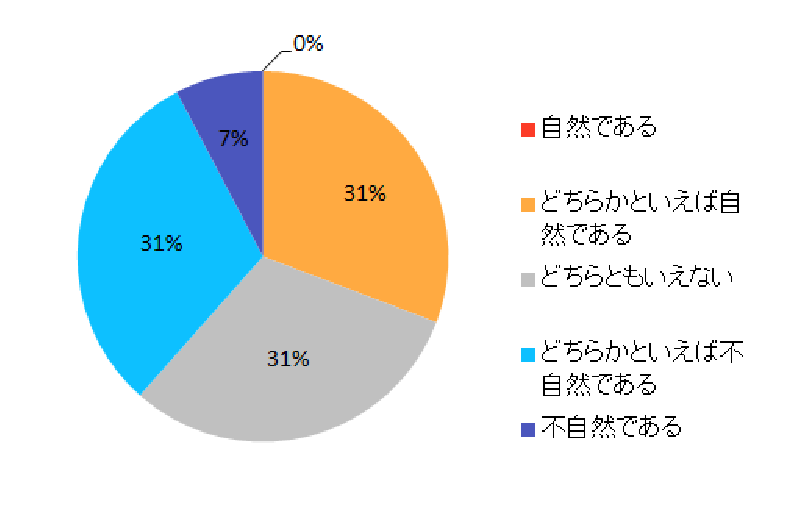
\includegraphics[width=4.8cm]{fig/chap4/Q1-4-2.eps}}
	\subcaptionbox{\textgt{楽器未経験者の回答}
		\label{fig:Q1-4-3}}{
		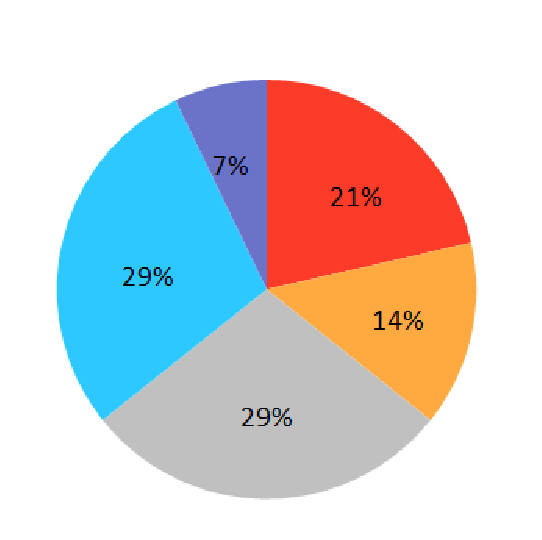
\includegraphics[width=4.8cm]{fig/chap4/Q1-4-3.eps}}
	\caption{トロンボーン奏者の身体の動きは自然か}
	\label{fig:Q1-4}
\end{figure}
%
%\newpage
\subsection{既存のアニメーションとの比較による評価}
既存の吹奏アニメーションにおける,トランペット奏者やトロンボーン奏者が実際に演奏しているシーンと,自動生成した吹奏アニメーションを比較することによる評価を,以下の4項目について行った.
\begin{itemize}
	\item トランペット奏者の指の動きは,どちらの方がより音楽のリズムに合っているか
	\item トランペット奏者の身体の動きは,どちらの方がより自然か
	\item トロンボーン奏者の腕の動きは,どちらの方がより音楽のリズムに合っているか
	\item トロンボーン奏者の身体の動きは,どちらの方がより自然か
\end{itemize}
\vspace{5mm}
\par
\figref{fig:Q2-1}は,既存のアニメーションと自動生成したアニメーションを比較したときに,トランペット奏者の指の動きはどちらの方がより音楽のリズムに合っているのかを評価した結果である.
吹奏楽やオーケストラ団体への所属経験や楽器の経験に関わらず,提案手法に対して肯定的な回答をした者が半数以上であった.
特に,吹奏楽やオーケストラ団体への所属経験者や金管楽器奏者は,ほとんどが肯定的な回答をした.
\begin{figure}[!h]
	\centering
	\subcaptionbox{\textgt{吹奏楽・オーケストラ団体への所属経験者または金管楽器経験者の回答}
		\label{fig:Q2-1-1}}{
		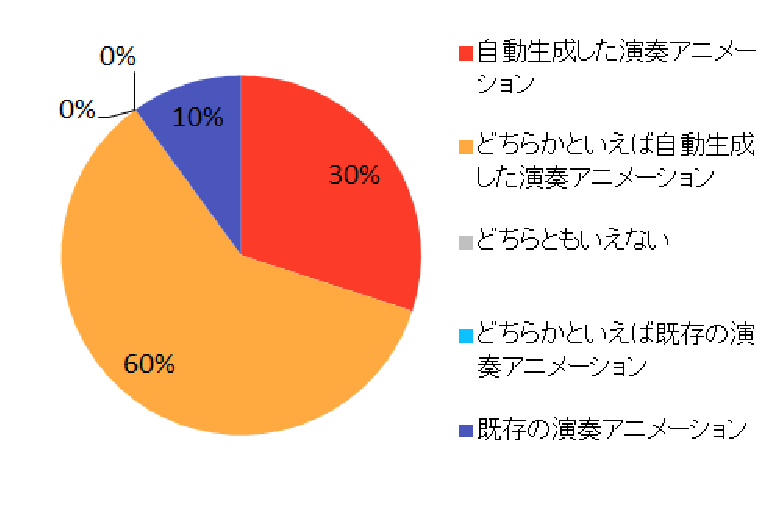
\includegraphics[width=4.8cm]{fig/chap4/Q2-1-1.eps}}
	\subcaptionbox{\textgt{(a)にはあてはまらない楽器経験者の回答}
		\label{fig:Q2-1-2}}{
		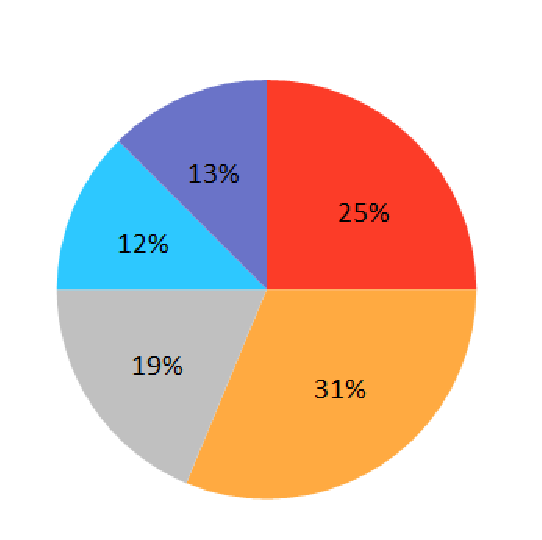
\includegraphics[width=4.8cm]{fig/chap4/Q2-1-2.eps}}
	\subcaptionbox{\textgt{楽器未経験者の回答}
		\label{fig:Q2-1-3}}{
		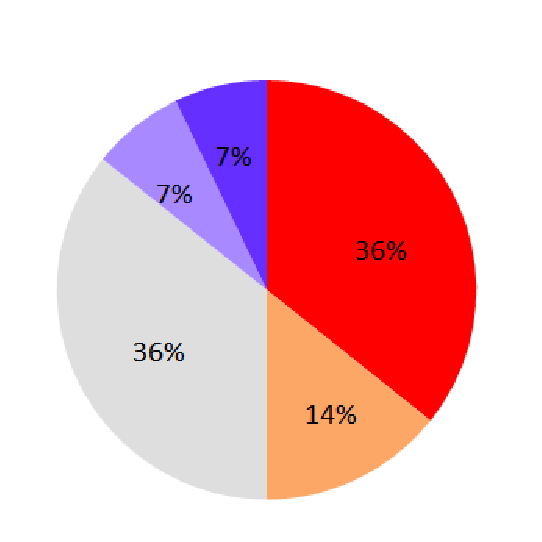
\includegraphics[width=4.8cm]{fig/chap4/Q2-1-3.eps}}
	\caption{既存のアニメーションと自動生成したアニメーションを比較したときに,トランペット奏者の指の動きは,どちらの方がより音楽のリズムに合っているか}
	\label{fig:Q2-1}
\end{figure}
\vspace{5mm}
\par
\figref{fig:Q2-2}は,既存のアニメーションと自動生成したアニメーションを比較したときに,トランペット奏者の身体の動きはどちらの方がより自然なのかを評価した結果である.
提案手法に対して肯定的な回答をした者はおらず,半数以上が否定的な回答をした.
\begin{figure}[!h]
	\centering
	\subcaptionbox{\textgt{吹奏楽・オーケストラ団体への所属経験者または金管楽器経験者の回答}
		\label{fig:Q2-2-1}}{
		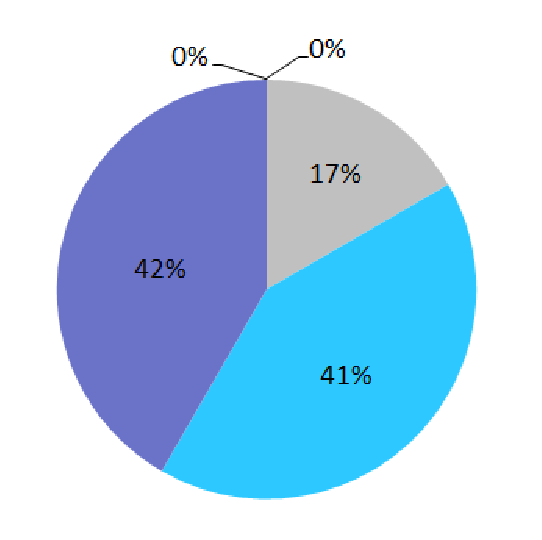
\includegraphics[width=4.8cm]{fig/chap4/Q2-2-1.eps}}
	\subcaptionbox{\textgt{(a)にはあてはまらない楽器経験者の回答}
		\label{fig:Q2-2-2}}{
		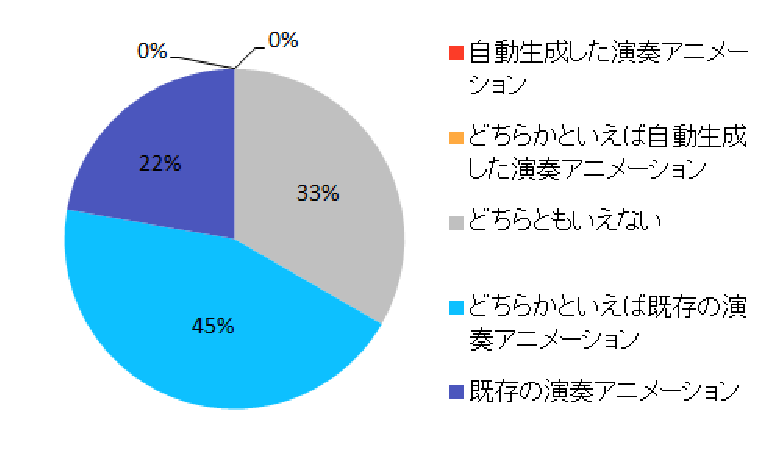
\includegraphics[width=4.8cm]{fig/chap4/Q2-2-3.eps}}
	\subcaptionbox{\textgt{楽器未経験者の回答}
		\label{fig:Q2-2-3}}{
		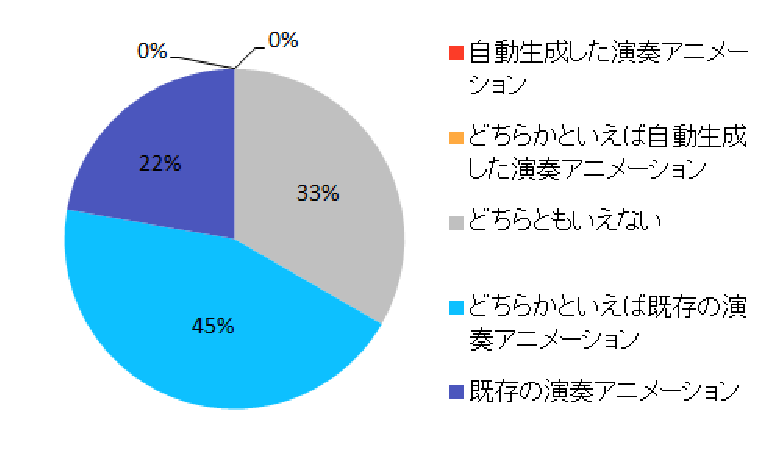
\includegraphics[width=4.8cm]{fig/chap4/Q2-2-3.eps}}
	\caption{既存のアニメーションと自動生成したアニメーションを比較したときに,トランペット奏者の身体の動きは,どちらの方がより自然か}
	\label{fig:Q2-2}
\end{figure}
\newpage
\par
\figref{fig:Q2-3}は,既存のアニメーションと自動生成したアニメーションを比較したときに,トロンボーン奏者の腕の動きはどちらの方がより音楽のリズムに合っているのかを評価した結果である.
吹奏楽やオーケストラ団体への所属経験や楽器の経験に関わらず,提案手法に対して肯定的な回答をした者が半数以上であった.
\figref{fig:Q2-1}とは異なり,肯定的な回答をした者の比率は,吹奏楽やオーケストラ団体への所属経験や楽器の経験によらなかった.
\begin{figure}[!h]
	\centering
	\subcaptionbox{\textgt{吹奏楽・オーケストラ団体への所属経験者または金管楽器経験者の回答}
		\label{fig:Q2-3-1}}{
		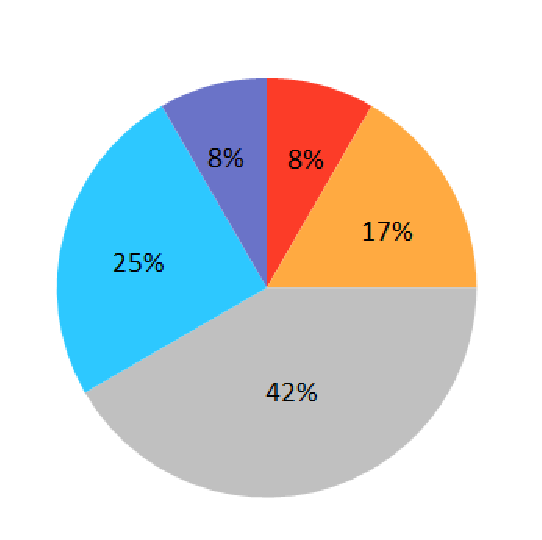
\includegraphics[width=4.8cm]{fig/chap4/Q2-3-1.eps}}
	\subcaptionbox{\textgt{(a)にはあてはまらない楽器経験者の回答}
		\label{fig:Q2-3-2}}{
		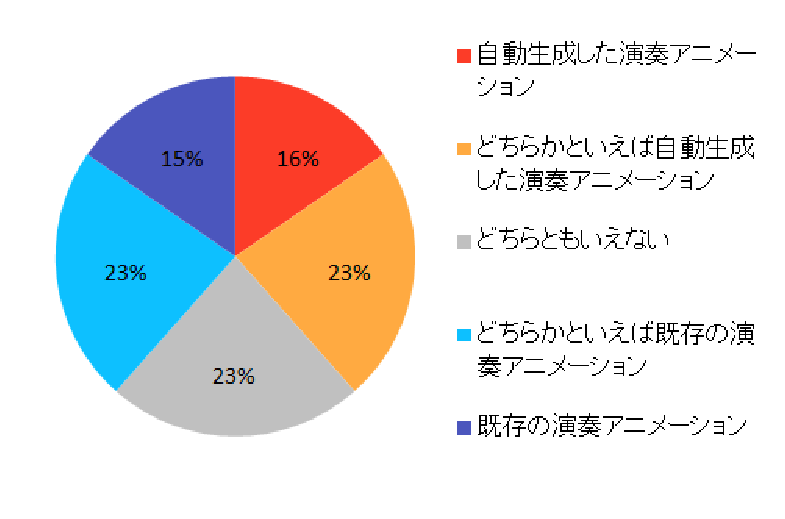
\includegraphics[width=4.8cm]{fig/chap4/Q2-3-2.eps}}
	\subcaptionbox{\textgt{楽器未経験者の回答}
		\label{fig:Q2-3-3}}{
		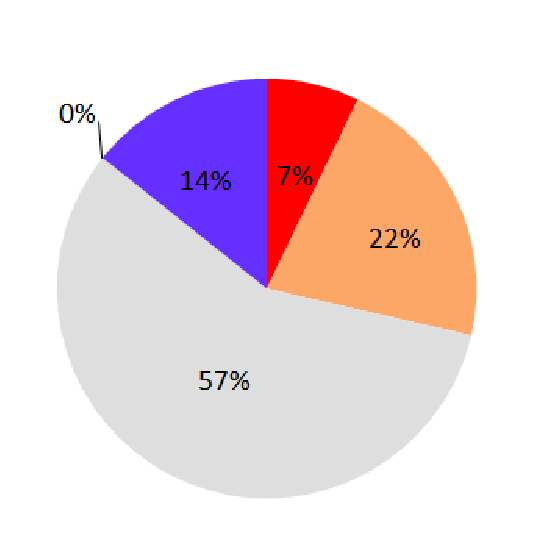
\includegraphics[width=4.8cm]{fig/chap4/Q2-3-3.eps}}
	\caption{既存のアニメーションと自動生成したアニメーションを比較したときに,トロンボーン奏者の腕の動きは,どちらの方が音楽のリズムに合っているか}
	\label{fig:Q2-3}
\end{figure}
\vspace{5mm}
\par
\figref{fig:Q2-4}は,既存のアニメーションと自動生成したアニメーションを比較したときに,トロンボーン奏者の身体の動きはどちらの方がより自然なのかを評価した結果である.
吹奏楽やオーケストラ団体への所属経験や楽器の経験がないほど,提案手法に対して肯定的な回答をした者の比率が高かった.
\begin{figure}[!h]
	\centering
	\subcaptionbox{\textgt{吹奏楽・オーケストラ団体への所属経験者または金管楽器経験者の回答}
		\label{fig:Q2-4-1}}{
		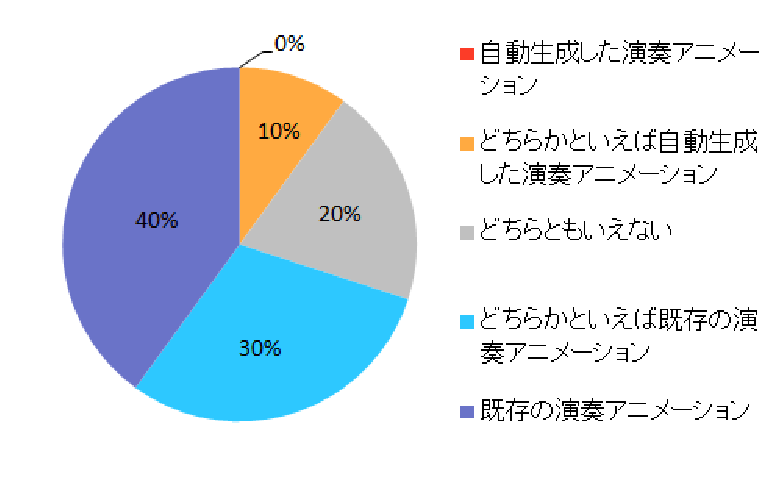
\includegraphics[width=4.8cm]{fig/chap4/Q2-4-1.eps}}
	\subcaptionbox{\textgt{(a)にはあてはまらない楽器経験者の回答}
		\label{fig:Q2-4-2}}{
		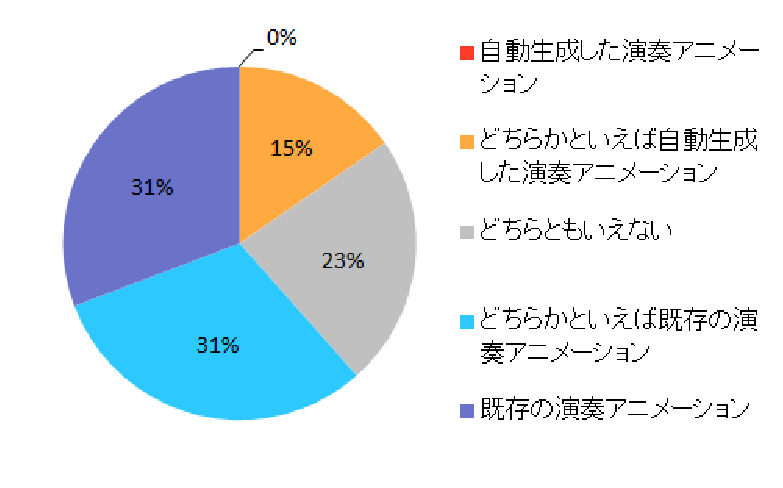
\includegraphics[width=4.8cm]{fig/chap4/Q2-4-2.eps}}
	\subcaptionbox{\textgt{楽器未経験者の回答}
		\label{fig:Q2-4-3}}{
		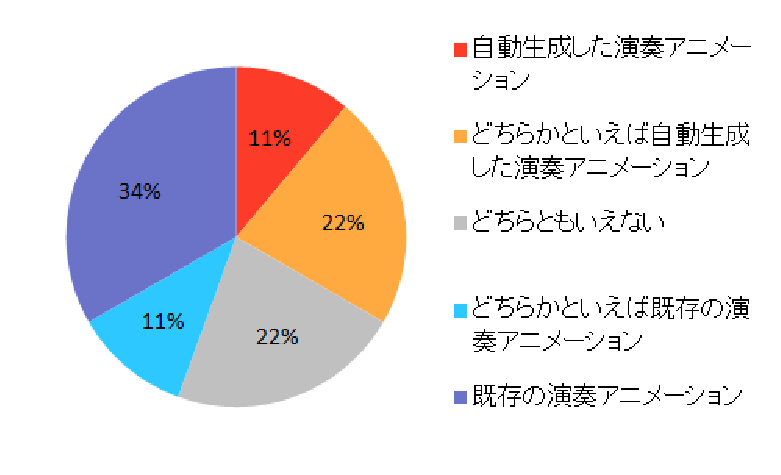
\includegraphics[width=4.8cm]{fig/chap4/Q2-4-3.eps}}
	\caption{既存のアニメーションと自動生成したアニメーションを比較したときに,トロンボーン奏者の身体の動きは,どちらの方がより自然か}
	\label{fig:Q2-4}
\end{figure}
\newpage
\subsection{アンサンブルアニメーションの評価}
自動生成したアンサンブルアニメーションの評価を,以下の2項目について行った.
\begin{itemize}
	\item 演奏時や息継ぎ時の口元は自然か
	\item 全員でタイミングを合わせつつ演奏している雰囲気はあるか
\end{itemize}
\par
\figref{fig:Q3-1}は,演奏時や息継ぎ時の口元は自然か否かを評価した結果である.
この項目については,金管楽器演奏者の口元の状態に関する知識のある者に対して評価を行ったため,回答者数はそれぞれ(a)9名,(b)9名,(c)7名となっている.
吹奏楽やオーケストラ団体への所属経験や,楽器の経験に関わらず,提案手法に対して肯定的な回答をした者の比率は,否定的な回答をした者の比率よりも高かった.
\begin{figure}[!h]
	\centering
	\subcaptionbox{\textgt{吹奏楽・オーケストラ団体への所属経験者または金管楽器経験者の回答}
		\label{fig:Q3-1-1}}{
		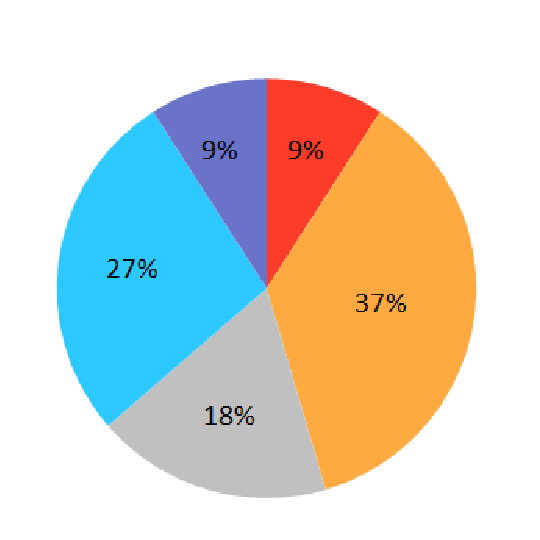
\includegraphics[width=4.8cm]{fig/chap4/Q3-1-1.eps}}
	\subcaptionbox{\textgt{(a)にはあてはまらない楽器経験者の回答}
		\label{fig:Q3-1-2}}{
		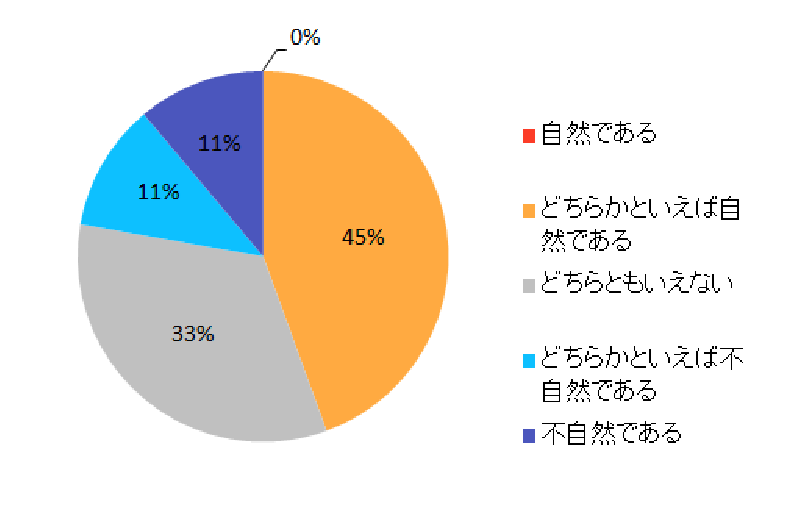
\includegraphics[width=4.8cm]{fig/chap4/Q3-1-2.eps}}
	\subcaptionbox{\textgt{楽器未経験者の回答}
		\label{fig:Q3-1-3}}{
		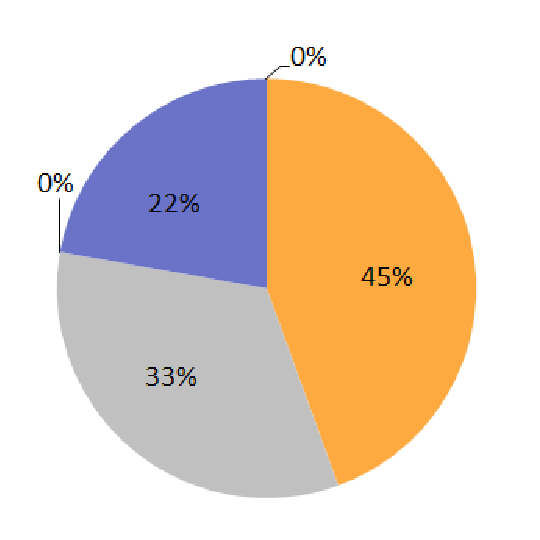
\includegraphics[width=4.8cm]{fig/chap4/Q3-1-3.eps}}	
	\caption{演奏時や息継ぎ時の口元は自然か}
	\label{fig:Q3-1}
\end{figure}
%\newpage
\par
\figref{fig:Q3-2}は,全員でタイミングを合わせつつ演奏している雰囲気があるか否かを評価した結果である.
吹奏楽やオーケストラ団体への所属経験者または金管楽器経験者のなかには,提案手法に対して否定的な回答をした者が少数いたが,それ以外はいなかった.
また,肯定的な回答をした者の比率は,吹奏楽やオーケストラ団体への所属経験や,楽器の経験がないほど高かった.
\begin{figure}[!h]
	\centering
	\subcaptionbox{\textgt{吹奏楽・オーケストラ団体への所属経験者または金管楽器経験者の回答}
		\label{fig:Q3-2-1}}{
		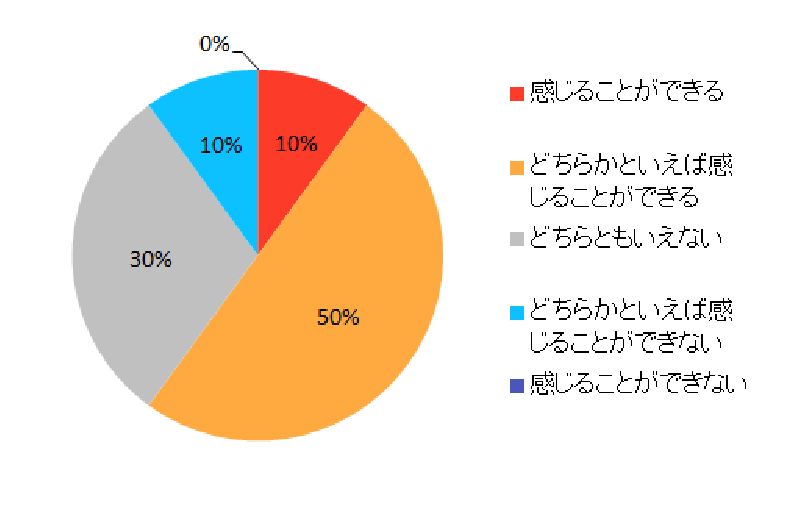
\includegraphics[width=4.8cm]{fig/chap4/Q3-2-1.eps}}
	\subcaptionbox{\textgt{(a)にはあてはまらない楽器経験者の回答}
		\label{fig:Q3-2-2}}{
		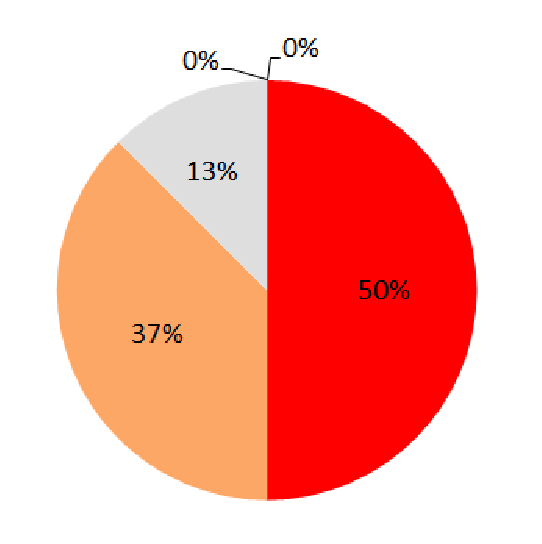
\includegraphics[width=4.8cm]{fig/chap4/Q3-2-2.eps}}
	\subcaptionbox{\textgt{楽器未経験者の回答}
		\label{fig:Q3-2-3}}{
		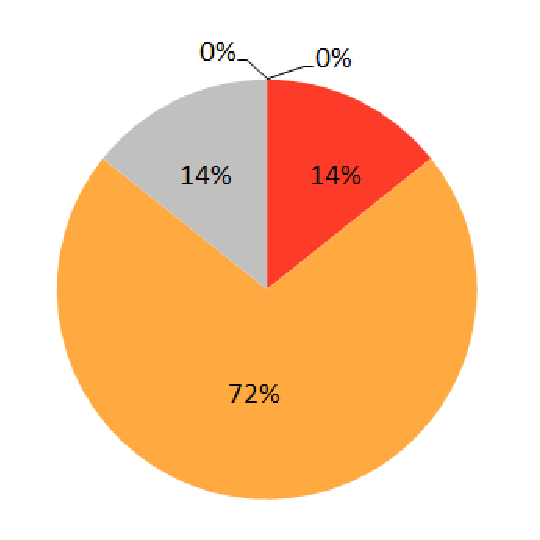
\includegraphics[width=4.8cm]{fig/chap4/Q3-2-3.eps}}	
	\caption{全員でタイミングを合わせつつ演奏している雰囲気はあるか}
	\label{fig:Q3-2}
\end{figure}
%
\newpage
\subsection{システムの有用性の予想}
アニメーション制作やCGに関する知識がある者15名に,本手法によりアニメーション制作時間や労力が軽減されると思うか否かを聞いた.
その結果,\figref{fig:ans2}のような結果を得た.全員が肯定的な回答をし,そのうち13名が軽減されると思うと回答したことから,本手法により,アニメータの制作支援が可能であると考えられる.
\begin{figure}[!h]
	\centering
	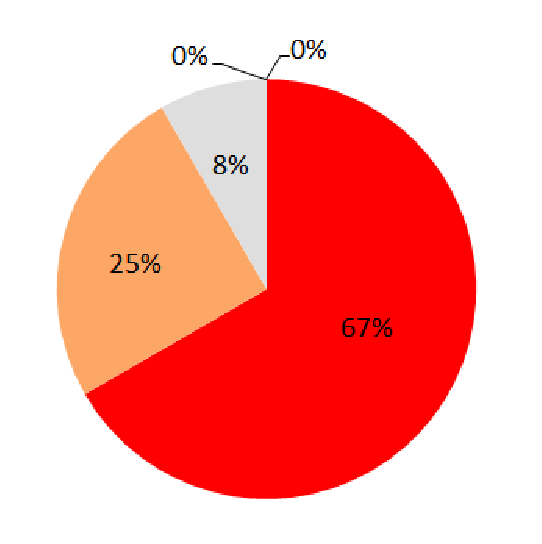
\includegraphics[width=6cm]{fig/chap4/Q1-1-1.eps}
	\caption{アニメーション制作の労力や時間が軽減されると思うか否か}
	\label{fig:ans2}
\end{figure}

\subsection{アンケート結果による本手法の総合的分析}
指や腕の動きのように,音楽情報から一意に決まる動きに関しては,本手法により音源に同期した自然なアニメーションが作成可能であるといえる.
一方,全身の動きのような個人差がある動きに関しては,現段階では本手法による自然なアニメーションが作成可能であるとはいえない結果となった.しかし,アニメータの作業支援は可能であると予想できる.\\
\indent
吹奏楽やオーケストラ団体への所属経験や楽器の経験がない者ほど,本手法に対して否定的な回答をした者の比率が高かった項目がある.
その要因として,グループによって自然だと感じる演奏の動作が異なっていることが挙げられると考えられる.